\documentclass[a4paper,12pt]{article}

\usepackage[utf8x]{inputenc}
\usepackage[english, russian]{babel}

\usepackage{tabularx}
\usepackage{multirow}
\usepackage{graphicx}
\usepackage{misccorr}
\usepackage{indentfirst}


\usepackage{listings}
\usepackage{xcolor}

\usepackage{fullpage}

\usepackage[labelsep=endash,
		    margin=10pt, 
		    justification = centerlast, 
		    format = hang,
		    singlelinecheck=false
		    ]{caption}

\exhyphenpenalty=10000
\doublehyphendemerits=10000
\finalhyphendemerits=5000

\definecolor{codegreen}{rgb}{0,0.6,0}
\definecolor{codegray}{rgb}{0.5,0.5,0.5}
\definecolor{codepurple}{rgb}{0.58,0,0.82}
\definecolor{backcolour}{rgb}{0.95,0.95,0.92}
 
\lstdefinestyle{mystyle}{
    backgroundcolor=\color{backcolour},
    commentstyle=\color{codegreen},
    keywordstyle=\color{blue},
    numberstyle=\tiny\color{codegray},
    stringstyle=\color{codepurple},
    basicstyle=\footnotesize,
    breakatwhitespace=false,
    breaklines=true,
    captionpos=t,
    keepspaces=true,
    numbers=left,
    numbersep=5pt,
    showspaces=false,
    showstringspaces=false
    showtabs=false,
    tabsize=4,
    frame=tb
}
 
\lstset{style=mystyle}

\usepackage{color}
\usepackage{xcolor}
\usepackage{listings}
 
% Цвета для кода
 
\definecolor{string}{HTML}{B40000} % цвет строк в коде
\definecolor{comment}{HTML}{008000} % цвет комментариев в коде
\definecolor{keyword}{HTML}{1A00FF} % цвет ключевых слов в коде
\definecolor{morecomment}{HTML}{8000FF} % цвет include и других элементов в коде
\definecolor{сaptiontext}{HTML}{FFFFFF} % цвет текста заголовка в коде
\definecolor{сaptionbk}{HTML}{999999} % цвет фона заголовка в коде
\definecolor{bk}{HTML}{FFFFFF} % цвет фона в коде
\definecolor{frame}{HTML}{999999} % цвет рамки в коде
\definecolor{brackets}{HTML}{B40000} % цвет скобок в коде
 

%%% Отображение кода %%%
 
% Настройки отображения кода
 
\lstset{
	%morekeywords={*,...}, % если хотите добавить ключевые слова, то добавляйте	 
	% Настройки отображения     
	breaklines=true, % Перенос длинных строк
	% Для отображения русского языка
	extendedchars=true,
	literate={Ö}{{\"O}}1
	{Ä}{{\"A}}1
	{Ü}{{\"U}}1
	{ß}{{\ss}}1
	{ü}{{\"u}}1
	{ä}{{\"a}}1
	{ö}{{\"o}}1
	{~}{{\textasciitilde}}1
	{а}{{\selectfont\char224}}1
	{б}{{\selectfont\char225}}1
	{в}{{\selectfont\char226}}1
	{г}{{\selectfont\char227}}1
	{д}{{\selectfont\char228}}1
	{е}{{\selectfont\char229}}1
	{ё}{{\"e}}1
	{ж}{{\selectfont\char230}}1
	{з}{{\selectfont\char231}}1
	{и}{{\selectfont\char232}}1
	{й}{{\selectfont\char233}}1
	{к}{{\selectfont\char234}}1
	{л}{{\selectfont\char235}}1
	{м}{{\selectfont\char236}}1
	{н}{{\selectfont\char237}}1
	{о}{{\selectfont\char238}}1
	{п}{{\selectfont\char239}}1
	{р}{{\selectfont\char240}}1
	{с}{{\selectfont\char241}}1
	{т}{{\selectfont\char242}}1
	{у}{{\selectfont\char243}}1
	{ф}{{\selectfont\char244}}1
	{х}{{\selectfont\char245}}1
	{ц}{{\selectfont\char246}}1
	{ч}{{\selectfont\char247}}1
	{ш}{{\selectfont\char248}}1
	{щ}{{\selectfont\char249}}1
	{ъ}{{\selectfont\char250}}1
	{ы}{{\selectfont\char251}}1
	{ь}{{\selectfont\char252}}1
	{э}{{\selectfont\char253}}1
	{ю}{{\selectfont\char254}}1
	{я}{{\selectfont\char255}}1
	{А}{{\selectfont\char192}}1
	{Б}{{\selectfont\char193}}1
	{В}{{\selectfont\char194}}1
	{Г}{{\selectfont\char195}}1
	{Д}{{\selectfont\char196}}1
	{Е}{{\selectfont\char197}}1
	{Ё}{{\"E}}1
	{Ж}{{\selectfont\char198}}1
	{З}{{\selectfont\char199}}1
	{И}{{\selectfont\char200}}1
	{Й}{{\selectfont\char201}}1
	{К}{{\selectfont\char202}}1
	{Л}{{\selectfont\char203}}1
	{М}{{\selectfont\char204}}1
	{Н}{{\selectfont\char205}}1
	{О}{{\selectfont\char206}}1
	{П}{{\selectfont\char207}}1
	{Р}{{\selectfont\char208}}1
	{С}{{\selectfont\char209}}1
	{Т}{{\selectfont\char210}}1
	{У}{{\selectfont\char211}}1
	{Ф}{{\selectfont\char212}}1
	{Х}{{\selectfont\char213}}1
	{Ц}{{\selectfont\char214}}1
	{Ч}{{\selectfont\char215}}1
	{Ш}{{\selectfont\char216}}1
	{Щ}{{\selectfont\char217}}1
	{Ъ}{{\selectfont\char218}}1
	{Ы}{{\selectfont\char219}}1
	{Ь}{{\selectfont\char220}}1
	{Э}{{\selectfont\char221}}1
	{Ю}{{\selectfont\char222}}1
	{Я}{{\selectfont\char223}}1
	{і}{{\selectfont\char105}}1
	{ї}{{\selectfont\char168}}1
	{є}{{\selectfont\char185}}1
	{ґ}{{\selectfont\char160}}1
	{І}{{\selectfont\char73}}1
	{Ї}{{\selectfont\char136}}1
	{Є}{{\selectfont\char153}}1
	{Ґ}{{\selectfont\char128}}1
	{\{}{{{\color{brackets}\{}}}1 % Цвет скобок {
	{\}}{{{\color{brackets}\}}}}1 % Цвет скобок }
}
\begin{document}

\begin{titlepage}
\newpage


\begin{center}
	\large		
   	Министерство образования и науки Российской Федерации\\[0.5cm]
    	
	ФГБОУ ВО Рыбинский государственный авиационный технический университет имени П.А. Соловьева\\[1.0cm]

	Факультет радиоэлектроники и информатики\\[0.25cm]
		
	Кафедра математического и программного обеспечения\\ электронных вычислительных средств\\[1.5cm]
	
	\Large
	\textbf{\textsc{ОТЧЕТ ПО ЛАБОРАТОРНОЙ РАБОТЕ №4}}\\[0.25cm]
	по  дисциплине\\
	\textbf{Тестирование и отладка\\ программного обеспечения}\\[0.5cm]
	
	по теме\\
	Системное тестирование
	
\end{center}

\vfill	
\begin{tabularx}{0.95\textwidth}{lXr}
Студенты группы ИПБ-13 			& &	Болотин Д. И.\\
								& &	Ивашин А.В. \\
Преподаватель к.т.н., ст. преп.	& & Воробьев К. А.\\
\end{tabularx}

\vspace{1.5cm}
\center Рыбинск 2016
\end{titlepage}	


\newpage
\setcounter{page}{2}

\tableofcontents

\newpage\section{Общее описание тестируемой системы}

Прект предназначен для шифрования/дешифрования текстов методами Моноалфавитной замены, Побитовой перестановки.
На рис. \ref{fig:class_diagram} представлена  диаграмма классов проекта.

\par После запуска программы пользователь видит окно авторизации (рис. \ref{fig:login_form}), с помощью которого он может либо авторизаоваться: введя логин (английский алфавит) и пароль; зарегистрироваться (рис. \ref{fig:registry_form}): введя информацию о себе и выбрав предпочтительные методы шифрования - представлены на интерфейсе двумя выпадающими списками (обязательными явлюятся поля: логин, пароль и методы шифрования, если в обоих выпадающих списках выбран один и тот же метод, то в БД попадает лишь один и пользователю будет доступна работа только с одним методом); либо же завершить работу с программой с помощью кнопки "Выход".
\begin{center}
	\begin{figure}[h!]
		\centering
   		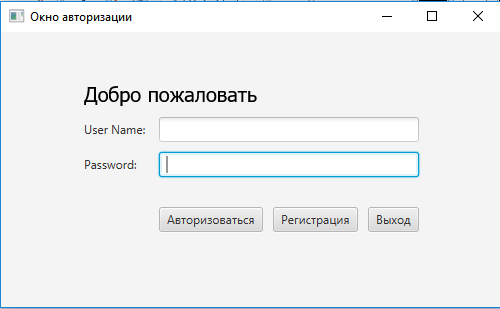
\includegraphics[scale=0.5]{img/login_form.png}
   		\caption{Окно авторизации}
   		\label{fig:login_form}
    \end{figure}
\end{center}
\begin{center}
	\begin{figure}[h!]
		\centering
   		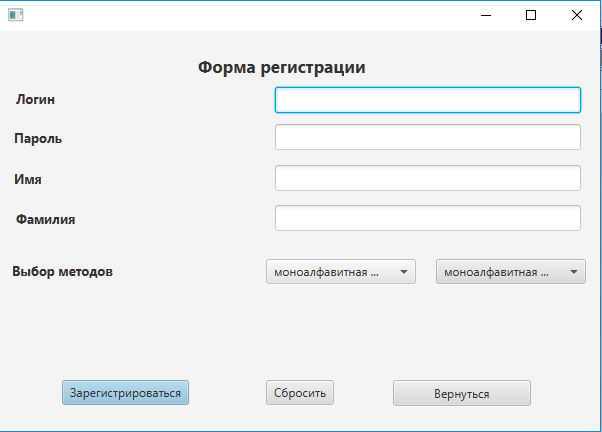
\includegraphics[scale=0.5]{img/registry_form.png}
   		\caption{Окно регистрации}
   		\label{fig:registry_form}
    \end{figure}
\end{center}
\par После прохождения авторизации пользователю открывается главное окно приложения, в котором ему, из списка методов шифрования, будут доступны лишь те методы, которые были выбраны им на этапе регистрации (рис. \ref{fig:main_form}).
\begin{center}
	\begin{figure}[h!]
		\centering
   		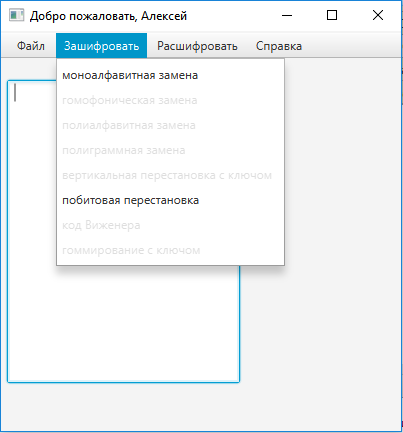
\includegraphics[scale=0.5]{img/main_form.png}
   		\caption{Главное окно программы}
   		\label{fig:main_form}
    \end{figure}
\end{center}

\begin{center}
	\begin{figure}[h!]
		\centering
   		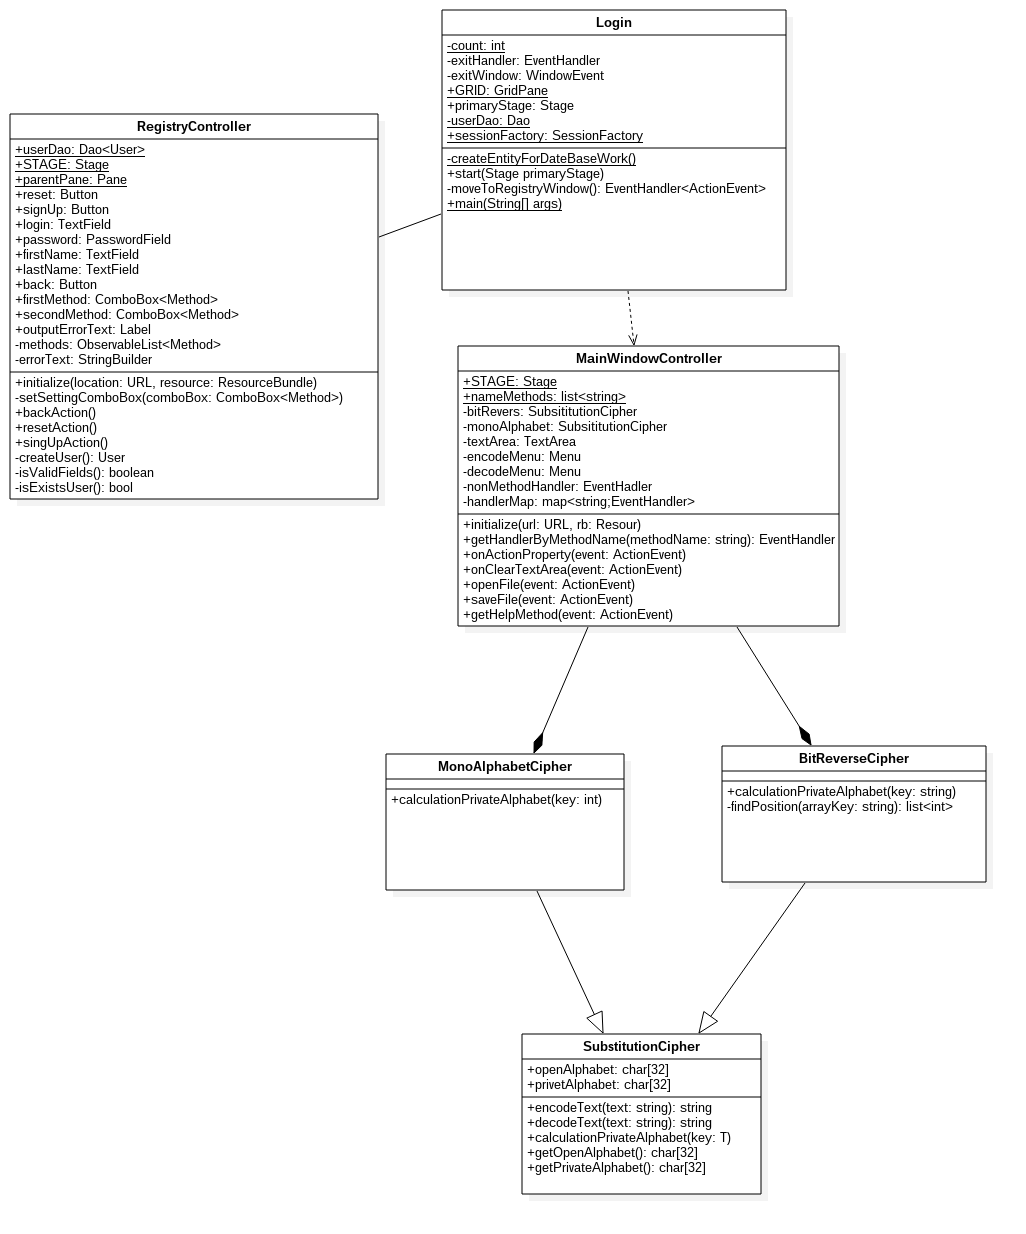
\includegraphics[scale=0.5]{img/class_diagram.png}
   		\caption{Диаграмма классов проекта}
   		\label{fig:class_diagram}
    \end{figure}
\end{center}

\subsection{Ограничения для шифруемого/расшифруемого текста}
Текст принимаемый методами шифрования состоит из строчных букв русского алфавита, из которого изключены буквы 'ё' и 'й', а так же пробел. Оставшиеся символы не входят в состав открытого алфавита, поэтому при их использовании в тексте пользователь увидит следующее сообщение: "Недопустимый символ. Расшифровка/Шифрование не возможно" (Последнее предложение зависит от выбранного пользователем метода. Пример на рис. \ref{fig:wrong_char_and_response}.
\begin{center}
	\begin{figure}[h!]
		\centering
		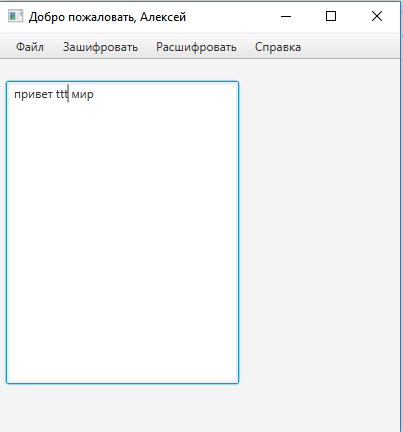
\includegraphics[scale=0.7]{img/wrong_char.png}
		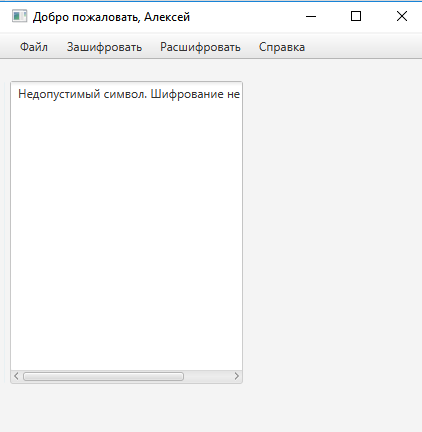
\includegraphics[scale=0.7]{img/wrong_char_response.png}
		\caption{Не верный символ в тексте}
		\label{fig:wrong_char_and_response}
	\end{figure}
\end{center}

\newpage\section{Общее описание тестирования}
В ходе данного тестирования проверяется работа пользовательского GUI как автоматизирванно (с помощью TestFx) так и в ручную. Проверяется работа приложения с базой данных, а также сохранение/загрузка текста в файл.

\par Для проведения тестирования использована библиотека JUnit, а также TestFX, которая нужна для моделирования взаимодействия пользователя с интерфейсом. Для проверки содержимого БД использовался просмотрщик БД ИСР IntellijIdea.

\newpage \section{Тестирование регистрации пользователя}
Протестируем работу GUI и работу с базой данных.  

\subsection{Попытка регистрации уже существующего пользователя}
Для начала проведём тестирования попытки регистрации пользователя, который уже есть в базе. Должно быть соответвующее сообщение. Класс для проведения этого тестирования представлен в листинге \ref{lstlisting_database:test_ui}.

\begin{lstlisting}[language=java, caption=код модуля DatabaseAndRegistryUiTest.java, label=lstlisting_database:test_ui]
package ui.RegistryUiTest;

import javafx.scene.control.Label;
import org.junit.Assert;
import org.junit.Test;
import ui.custom.LoginUiCustomTest;

import static org.loadui.testfx.GuiTest.find;

/**
 * Created by Алексей on 26.12.2016.
 */
public class DatabaseAndRegistryUiTest extends LoginUiCustomTest {

    @Test
    public void userExistsTest() {
        clickOn(registry);
        clickOn("#login").write("Aleksey");
        clickOn("#password").write("tesPass");
        clickOn("#signUp");
        Label outputErrorText = find("#outputErrorText");
        Assert.assertEquals(outputErrorText.getText(), "Пользователь с логином: Aleksey существует!");
        closeRegistryWindowAndTest();
    }


}
\end{lstlisting}

\subsection{Добавление пользователя в БД}
\par Сценарий тестирования регистрации пользователя заключается в следующем:
\begin{enumerate}
\item На форме авторизации нажатие кнопки "Регистрация".
\item Запоняем все поля формы, предварительно убедившись, что такого пользователя нет в базе.
\item Нажимаем на кнопку регистрация и убеждаемся, что в БД плявилась соответствующая запись. При этом с формы ргистрации мы должны обратно прейти к форме авторизации.
\item Вводим логин и пароль нового пользователя после чего должны попасть на главное окно.
\item Убеждаемся, что активированы только те методы, которые были указаны при регистации.
\end{enumerate}

\newpage \section{Тестирвоание загрузки и сохранения в файл}
Тестирование проводится вручную  по следущему сценарию:
\begin{enumerate}
\item Авторизуемся.
\item Пишем в поле ввода "Текст для записи в файл".
\item В меню выбираем Файл->Сохранить.
\item Убедимся, что файл был создан.
\item В меню выбираем Файл->Загрузить.
\item Убедимя, что файл загружен правильно.
\end{enumerate}

\newpage \section{Пример тестирования}

В таблицах \ref{table:data_type1} - \ref{table:data_type5}, приведены примеры выполнения ручных сценариев тестирования.

\begin{table}[h]
	\caption{Тестрование регистрации пользователя}
	\centering
	\begin{tabular}{|c|c|c|}
	\hline 
	№  & Результат & Примечание \\ 
	\hline 
	1 & 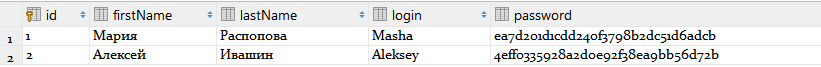
\includegraphics[scale=0.3]{img/database/before_registry_user.png} & В базе присутсвуют \\ && только два пользователя \\
	\hline 
	2 & 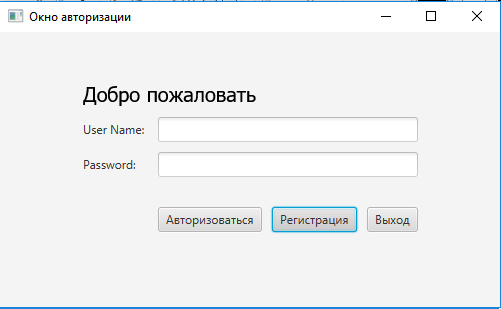
\includegraphics[scale=0.3]{img/database/before_registry_methods.png} & В базе каждому пользователю \\ && соответсвуют два метода\\
	\hline 
	3 & 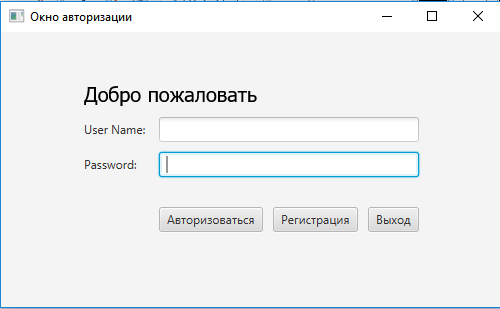
\includegraphics[scale=0.3]{img/login_form.png} & Открываем окно авторизации\\
	\hline 
	4 & 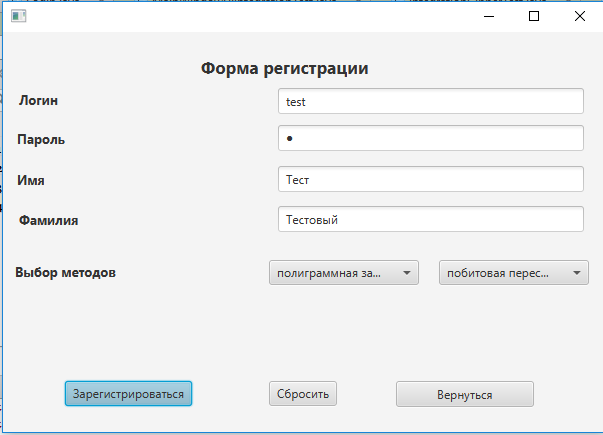
\includegraphics[scale=0.3]{img/database/before_registry_form.png} & Открываем окно регистрации \\ && и заполняем все поля\\
	\hline 
	5 & 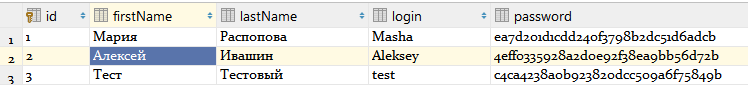
\includegraphics[scale=0.3]{img/database/after_registry_user.png} & После регистрации можно увидеть, \\ && что введенный пользователь появился в БД\\
	\hline
\end{tabular} 
\label{table:data_type1} 
\end{table}

\begin{table}[pt!]
	\caption{Тестрование регистрации пользователя}
	\centering
	\begin{tabular}{|c|c|c|}
	\hline 
	№  & Результат & Примечание \\ 
	\hline 
	6 & 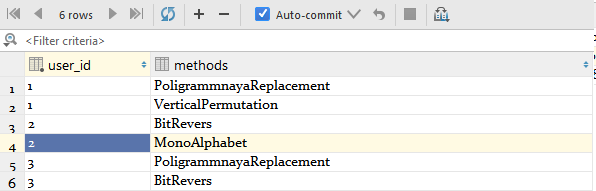
\includegraphics[scale=0.3]{img/database/after_registry_methods.png} & Так же можно увидеть, что \\ && для нового пользователя \\ && появились соответсвующие методы\\
	\hline 
	7 & 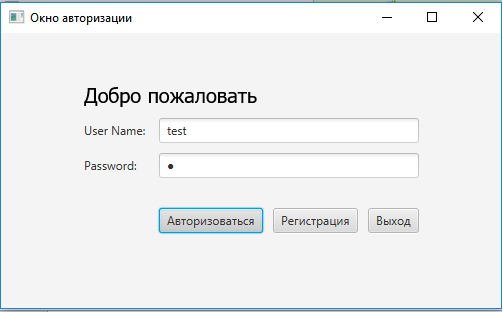
\includegraphics[scale=0.3]{img/database/authorization.png} & Открываем окно авторизации \\ && и заходим в систему под \\ && новым пользователем\\
	\hline 
	8 & 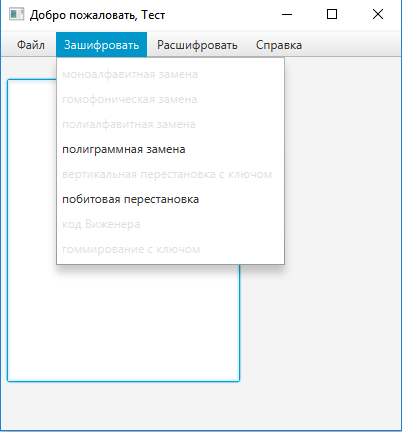
\includegraphics[scale=0.3]{img/database/main_open_methods.png} & Так же можно увидеть, \\ && что для нового пользователя появились\\ &&  соответсвующие методы шифрования\\
	\hline 
	9 & 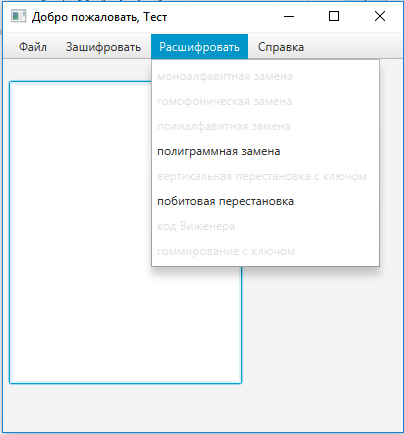
\includegraphics[scale=0.3]{img/database/main_open_methods2.png} & Так же можно увидеть, \\ && что для нового пользователя появились\\ &&  соответсвующие методы расшифрования\\
	\hline 
\end{tabular} 
\label{table:data_type2} 
\end{table}

\begin{table}[pt!]
	\caption{Тестрование сохранения в файл}
	\centering
	\begin{tabular}{|c|c|c|}
	\hline 
	№  & Результат & Примечание \\ 
	\hline 
	1 & 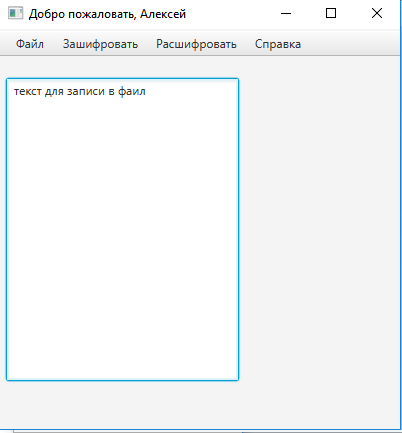
\includegraphics[scale=0.3]{img/file/open/text_open4.png} & Вводим текст в поле для \\ && ввода текста (memo) \\
	\hline 
	2 & 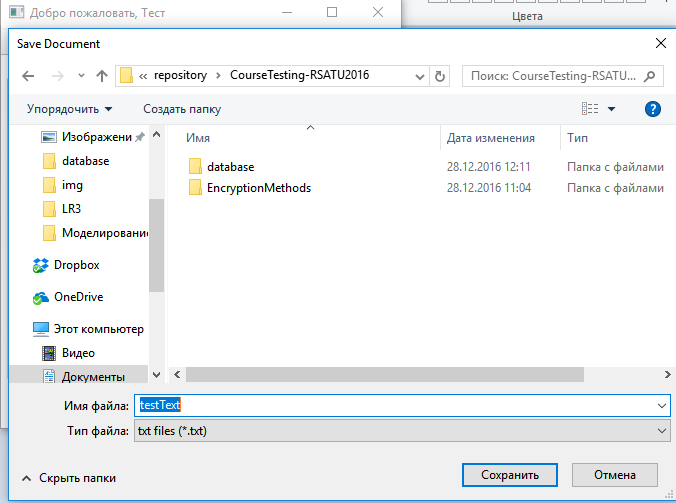
\includegraphics[scale=0.3]{img/file/save/text_path.png} & Выбираем путь, куда будет \\ && сохранен файл с текстом\\
	\hline 
	3 & 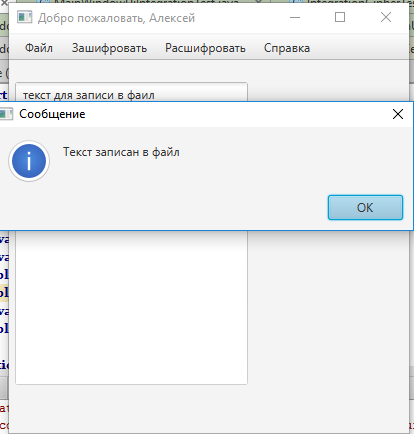
\includegraphics[scale=0.3]{img/file/save/text_okey_save.png} & Вывод сообщения о том что файл сохранен\\
	\hline 
\end{tabular} 
\label{table:data_type3} 
\end{table}

\begin{table}[pt!]
	\caption{Тестрование открытия файла}
	\centering
	\begin{tabular}{|c|c|c|}
	\hline 
	№  & Результат & Примечание \\ 
	\hline 
	1 & 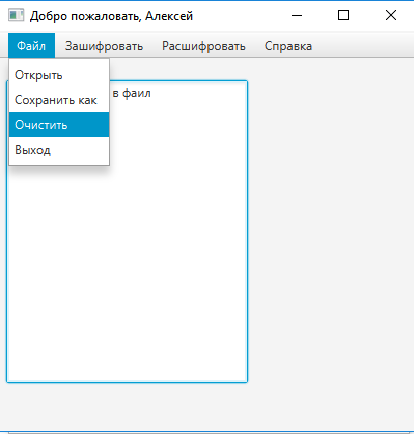
\includegraphics[scale=0.3]{img/file/open/text_clear.png} & Выбираем очистку поля ввода \\
	\hline 
	2 & 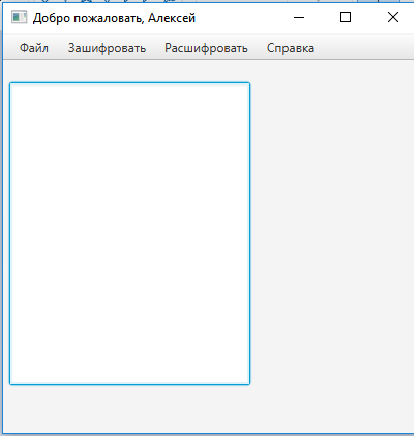
\includegraphics[scale=0.3]{img/file/open/text_clear1.png} & Видим что поле очистилось\\
	\hline 
	3 & 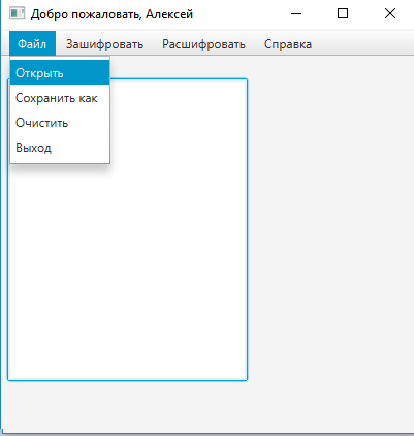
\includegraphics[scale=0.3]{img/file/open/text_open.png} & Выбираем открытие файла\\
	\hline 
\end{tabular} 
\label{table:data_type4} 
\end{table}
\begin{table}[pt!]
	\caption{Тестрование открытия файла}
	\centering
	\begin{tabular}{|c|c|c|}
	\hline 
	№  & Результат & Примечание \\ 
	\hline 
	5 & 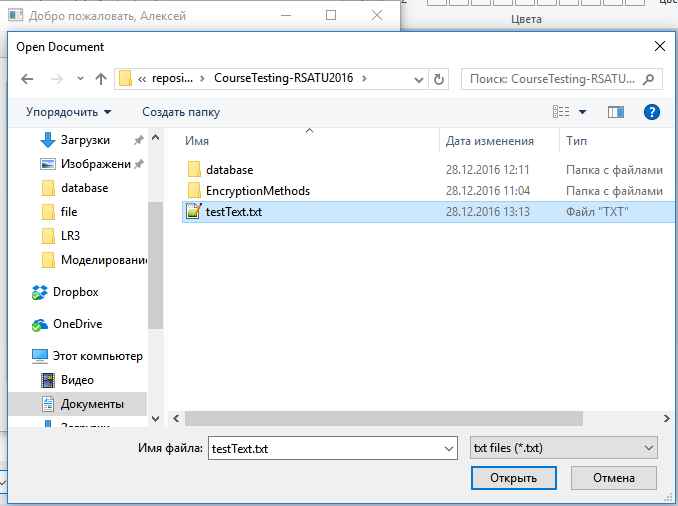
\includegraphics[scale=0.3]{img/file/open/text_open2.png} & Выбираем путь до файла\\
	\hline 
	6 & 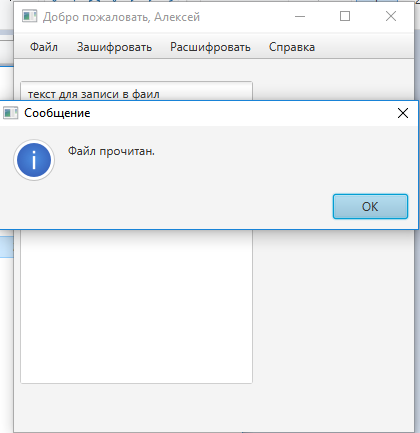
\includegraphics[scale=0.3]{img/file/open/text_open3.png} & Видим, что файл открылся\\
	\hline
	7 & 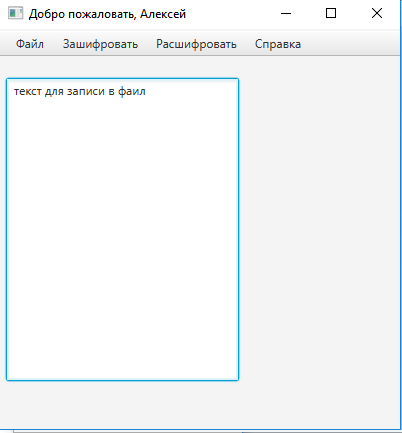
\includegraphics[scale=0.3]{img/file/open/text_open4.png} & Текст из файла в поле\\
	\hline
\end{tabular} 
\label{table:data_type5} 
\end{table}

\newpage\section*{Выводы}
\addcontentsline{toc}{section}{Выводы}
В ходе выполнения лабораторной работы было разработано и проведено системное тестирвание пректа. Для написания тестов была использована библиотека JUnit, а действия пользователя моделировались с помошью библиотеки TestFX. Ручные тесты составлялись из рассчёта на то, чтобы смоделировать типовые действие пользователя, которые не были протестированы на предыдущем этапе. В ходе тестирования ошибок не обнаружено.


\end{document}